
\documentclass[a4paper, 12p]{paper} 
\usepackage[margin=2.5cm]{geometry}
\usepackage{amsmath}
\usepackage{graphicx}
\usepackage{lipsum}
\usepackage{xcolor}
\usepackage{booktabs}
\usepackage{float}
\usepackage{subfigure}
\usepackage{titling}
\usepackage{kotex}
\usepackage{gensymb}

\def\code#1{\texttt{#1}}
\sectionfont{\large\sf\bfseries\color{black!70!blue}}
\date{\vspace{-5ex}}
\renewcommand{\familydefault}{\sfdefault}
\renewcommand{\baselinestretch}{1.3} 

\pretitle{\centering\LARGE\bfseries}
\posttitle{\par}
\preauthor{\begin{flushright}\large}
\postauthor{\end{flushright}}

\title{Affine Transform of Digital images}
\author{전자공학과 20161453 김규래}

\begin{document} 
\maketitle\hrule{}\bigskip

\section{Overview}
Affine matrix 를 이용한 영상들의 geometric transformation 을 직접 구현하는 것이 본 과제의 목표이다. 이 구현에서는 C++ 만을 사용하였으며 입출력과 선형대수학 연산을 위해서 일부 외부 라이브러리들을 사용하였다. Affine transformation 은 선형변환에 기저변환 (basis transformation) 을 조합한 $y = Ax + b$ 형태로 표현이 되는데, 본 과제에서는~\ref{eq:augmentation} 형태로 augmentation matrix 를 사용하여 affine transformation 을 구현하였다.

\begin{equation}
  \left(
  \begin{array}{c}
    y \\
    1
  \end{array}
  \right)
  =
  \left(
  \begin{array}{c|c}
    A & b \\
    0 & 1
  \end{array}
  \right)
  \left(
  \begin{array}{c}
    x \\
    1
  \end{array}
  \right)\label{eq:augmentation}
\end{equation}

이 때 $x$ 와 $y$ 는 각각 영상이 되며, \textit{augmented affine transformation matrix} (AugATM) 는 $T$ 로 부르도록 하겠다. 이제부터 Affine transformation 은 $y = Tx$ 가 된다. $x$ 와 $y$ 는 어떠한 continuous domain 속의 영상 $\hat{x}$ 과 $\hat{y}$ 를 샘플링한 후 discretize 한 discrete domain 이미지로 생각할 수 있다. Discrete domain 에서의 영상은 정보가 불완전하기 때문에 $x$ 와 $y$ 의 변환 과정에서 정보의 손실이 존재한다. 이를 보완하기 위해서 원래의 연속 영상을 근사하는 interpolation 작업이 필요하게 된다. 본 구현에서는 다음과 같은 interpolation 기법들을 구현하였다.

\begin{itemize}
  \item Nearest neighbor
  \item Bilinear 
  \item Bicubic
\end{itemize}

\subsection{Forward and Inverse Mapping}
두 discrete domain 간의 affine transformation을 진행할 때 정보가 존재하지 않는 윈치에 픽셀값이 필요한 경우가 발생한다. 특히 $y = Tx$ 변환에 대해서 forward mapping 방식을 선택할 경우에는 $Tx$ 의 도메인에서 이러한 문제가 발생하게 되는데, 이 때 interpolation 작업을 진행하기 위해서는 $Tx$ 도메인에서 다수의 픽셀 정보들을 갖고 있어야 한다. 이는 구현을 할 때 $x$ 와 $Tx$ 의 정보를 모두 갖고 있어야 함을 의미하며, 추가적인 메모리를 필요로 하게 된다. 반면에 inverse mapping 또는 backward mapping 을 사용할 경우에는 $yT^{-1} = x$ 와 같은 형태로 연산을 수행하는데 $yT^{-1}$ 의 도메인에서 interpolation 을 한다. $yT^{-1}$ 도메에서의 interpolation은 곧 $x$ 를 이용하므로 forward mapping 에 비해서 메모리를 적게 필요로 한다. 또한 이러한 작업이 forward mapping 에 비해서 보통 덜 복잡하게 구현이 가능하다는 장점도 있다. 정리하자면, 다음과 같은 이유로 inverse mapping 이 forward mapping 에 비해서 구현이 더 유리하다:

\begin{itemize}
  \item interpolation 을 진행할 때 메모리를 덜 소모한다.
  \item 구현이 상대적으로 단순하다.
\end{itemize}

\section{Implementation}
언어는 C++14 를 사용하였으며 빌드 시스템은 CMake 로 구성하였다. 리눅스 환경에 맞게 작성이 됐기 때문에 리눅스에서 빌드할 것을 권장한다.

\subsection{External Dependencies}
외부 라이브러리로는 OpenCV\footnote{https://opencv.org/} 와 Blaze\footnote{https://bitbucket.org/blaze-lib/blaze}를 사용하였다. OpenCV 에서는 다양한 영상처리 관련 루틴들을 제공하고 있으나, 본 과제에서는 \code{cv::imshow()} 와 \code{cv::imread()}, \code{cv::imwrite()} 와 같은 입출력 관련 함수들만 사용하였다. Blaze 는 C++ 선형대수학 라이브러리로, 행렬-벡터곱을 위해서 사용하였다.

\subsection{Installation}
시스템에 OpenCV 가 표준 경로에 설치돼있을 경우 CMake 에서 자동으로 인식을 할 것이다. 별도의 경로에 설치돼 있을 경우 \code{OpenCV\_ROOT\_DIR} 변수를 CMake 에 플래그로 넘김으로써 경로를 알려줄 수 있다. Blaze 의 경우에는 함께 첨부돼 있기 때문에 별도의 작업이 필요하지 않다. 다음과 같이 입력하면 빌드를 할 수 있다. 

\begin{align*}
  & \code{mkdir build \&\& cd build} \\
  & \code{cmake -G ``Unix Makefiles'' ..} \\
  & \code{make}
\end{align*}

\subsection{Affine Transformation}
각 구현에서는 다음과 같은 AugATM 를 사용하였다. 모두 inverse transform 형태로 구현이 됐으므로 실제로는 $y=Tx$ 에서의 $T$ 가 아니라 그 역변환인 $T^{-1}$ 에 해당한다.

\subsection{구현1}
다음 AugATM $T_1$은 입력 영상을 $1/8$ 로 축소한다.

\begin{equation}
  T_1^{-1} = 
  \begin{pmatrix}
    8 & 0 & 0 \\
    0 & 8 & 0 \\
    0 & 0 & 1
  \end{pmatrix}
\end{equation}

다음 AugATM $T_2$은 입력 영상을 $8$ 배로 확대한다. 위의 연산을 이용해 축소된 영상을 다시 확대하는 역할을 한다.
\begin{equation}
  T_2^{-1} = 
  \begin{pmatrix}
    1/8 & 0   & 0 \\
    0   & 1/8 & 0 \\
    0   &  0  & 1
  \end{pmatrix}
\end{equation}

\subsection{구현2}
다음 AugATM $T$는 입력 영상을 15도 회전시킨 다음 $x$축을 따라 +10 픽셀, $y$ 축을 따라 +20 픽셀 이동시킨다.

\begin{equation}
  T^{-1} = 
  \begin{pmatrix}
    \cos(-15 \degree)  & \sin(-15 \degree) & -10 \\
    -\sin(-15 \degree) & \cos(-15 \degree) & -20 \\
    0                  & 0                 & 1 
  \end{pmatrix}
\end{equation}

\subsection{Performance}
C++ 로 구현한 affine transformation 의 성능을 간단하게 측정해보았다. 결과는 Fig.~\ref{fig:throughput} 에서 볼 수 있다.

\begin{figure}[H]
\centering
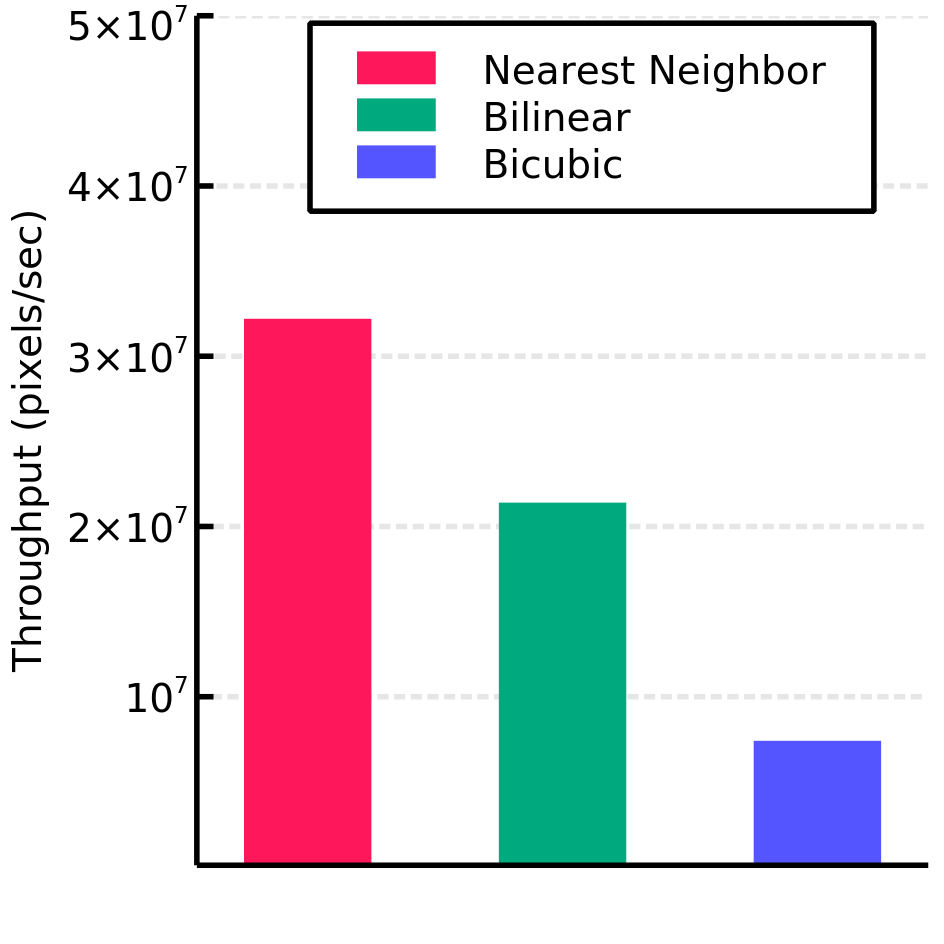
\includegraphics[scale=0.45]{../data/throughput.png}
\caption{구현한 코드의 초당 픽셀 처리량.}
\label{fig:throughput}
\end{figure}

쉽게 예상할 수 있듯이, Nearest Neighbor 의 경우에는 인접한 4개의 픽셀들 간의 거리를 계산한 후, 거리를 비교하면 되기 때문에 가장 연산량이 적다. 본 구현체에서는 거리를 잴 때 $L1$-distance 를 사용하였다. Bilinear interpolation 의 경우에는 인접한 4개의 픽셀로 2번의 linear line fitting 을 진행하고, bicubic interpolation 의 경우에는 인접한 16개의 픽셀에 접근한 다음에 총 5번의 $3^{rd}$ order curve fitting 을 진행한다. 따라서 bicubic 이 연산량이 제일 많고, 이러한 사실은 bicubic 의 pixel throughput 이 제일 낮다는 점에서 확인할 수 있다.

\subsection{Border Padding}
Interpolation 을 수행할 때 인접한 4개 또는 16개의 픽셀들의 값을 참조하게 되는데, 그러한 정보가 존재하는 영역이 영상보다 좁기 때문에 정보의 부족이 발생한다. 이 문제를 해결하기 위해서는 영상의 가장자리를 연장하는 padding 을 하는데 본 구현에서는 padding 을 해야하는 값과 가장 가까운 픽셀을 복사하는 border replication padding 을 적용하였다.

\section{Results}
\subsection{구현1}

구현1 에서는 제공받은 영상 \code{Chronometer.tif} 을 8배 축소한 다음 8배 확대한 뒤 원본 영상과 비교를 해보았다. 연산을 수행한 결과물은 Fig.~\ref{fig:result1} 에서 확인할 수 있다. Nearest neighbor 의 경우에는 굉장히 경계선들이 거친 점묘화 비슷한 영상이 나온 것을 확인할 수 있으며, bilinear 를 사용한 경우에는 조금 더 부드러운 영상이 나온 것을 볼 수 있다. Bicubic 방식을 사용한 결과물의 경우 bilinear 와 유사하나 조금 더 선명도가 올라간 것을 확인할 수 있다.

각각의 absolute difference 를 구한 차영상을 구할 경우 Fig.~\ref{fig:diff} 와 같다. 차영상을 비교할 때는 bilinear 와 bicubic 을 사용했을 때는 큰 차이가 보이지 않으나 nearest neighbor 방식을 사용한 것은 차이가 큰 부분들이 네모낳게 형성되는 것을 확인할 수 있다. 이를 볼 때 nearest neighbor 방식이 다른 방식들에 비해서 오차가 크다는 것을 추정해볼 수 있다.

\begin{figure}[H]
\centering
\subfigure[Nearest Neighbor]{
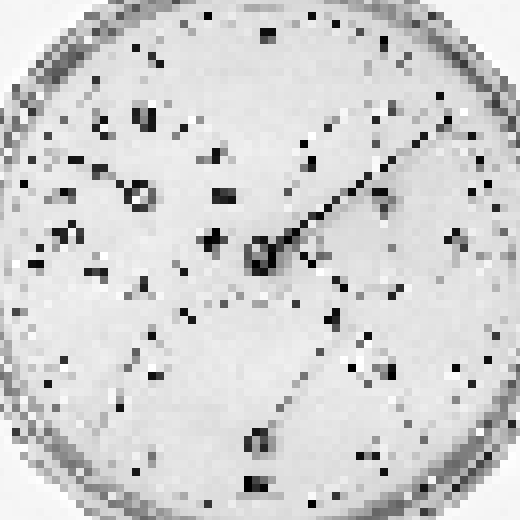
\includegraphics[scale=0.25]{../data/nearest_impl1.png}
}
\subfigure[Bilinear]{
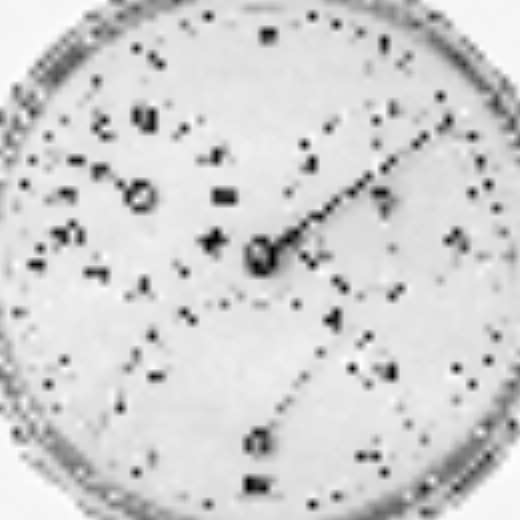
\includegraphics[scale=0.25]{../data/bilinear_impl1.png}
}
\subfigure[Bicubic]{
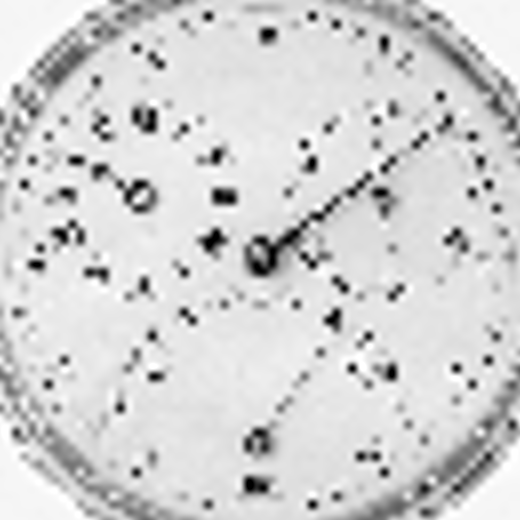
\includegraphics[scale=0.25]{../data/bicubic_impl1.png}
}
\caption{(a) Nearest neighbor, (b) bilinear, (c) bicubic interpolation 을 사용한 결과물.}
\label{fig:result1}
\end{figure}

\begin{figure}[H]
\centering
\subfigure[Nearest Neighbor]{
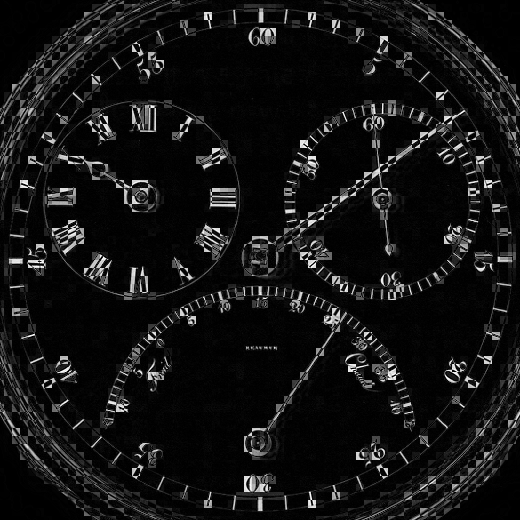
\includegraphics[scale=0.25]{../data/diff_nearest_impl1.png}
}
\subfigure[Bilinear]{
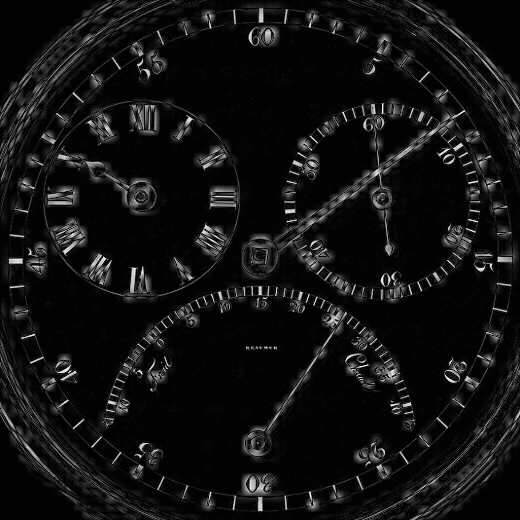
\includegraphics[scale=0.25]{../data/diff_bilinear_impl1.png}
}
\subfigure[Bicubic]{
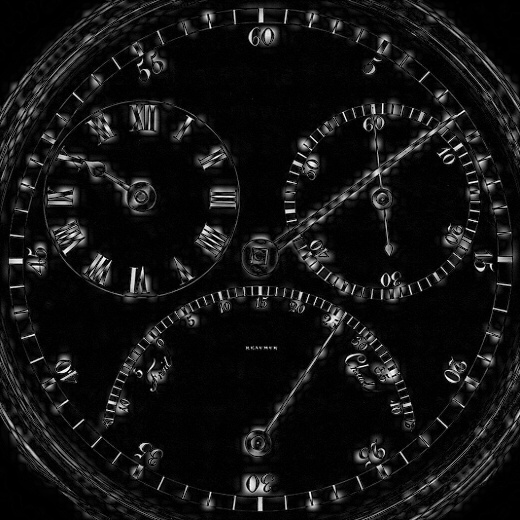
\includegraphics[scale=0.25]{../data/diff_bicubic_impl1.png}
}
\caption{(a) Nearest neighbor, (b) bilinear, (c) bicubic interpolation 을 사용했을 때의 차영상.}
\label{fig:diff}
\end{figure}

각 방식의 오차를 정량적으로 파악하기 위해서 영상들의 \textit{peak signal-to-noise ratio} (PSNR) 를 구해볼 경우 Fig.~\ref{fig:psnrx8} 와 같다.

\begin{figure}[H]
\centering
\subfigure[8배]{
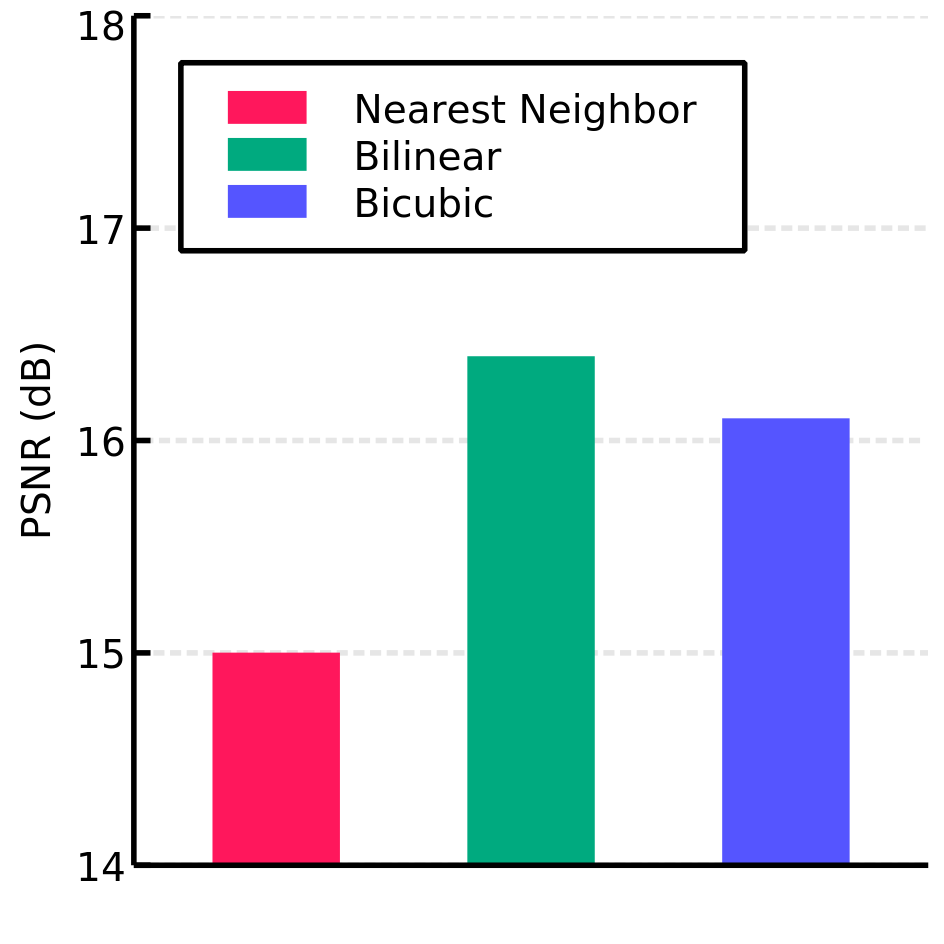
\includegraphics[scale=0.45]{../data/psnr_x8.png}\label{fig:psnrx8}
}
\subfigure[4배]{
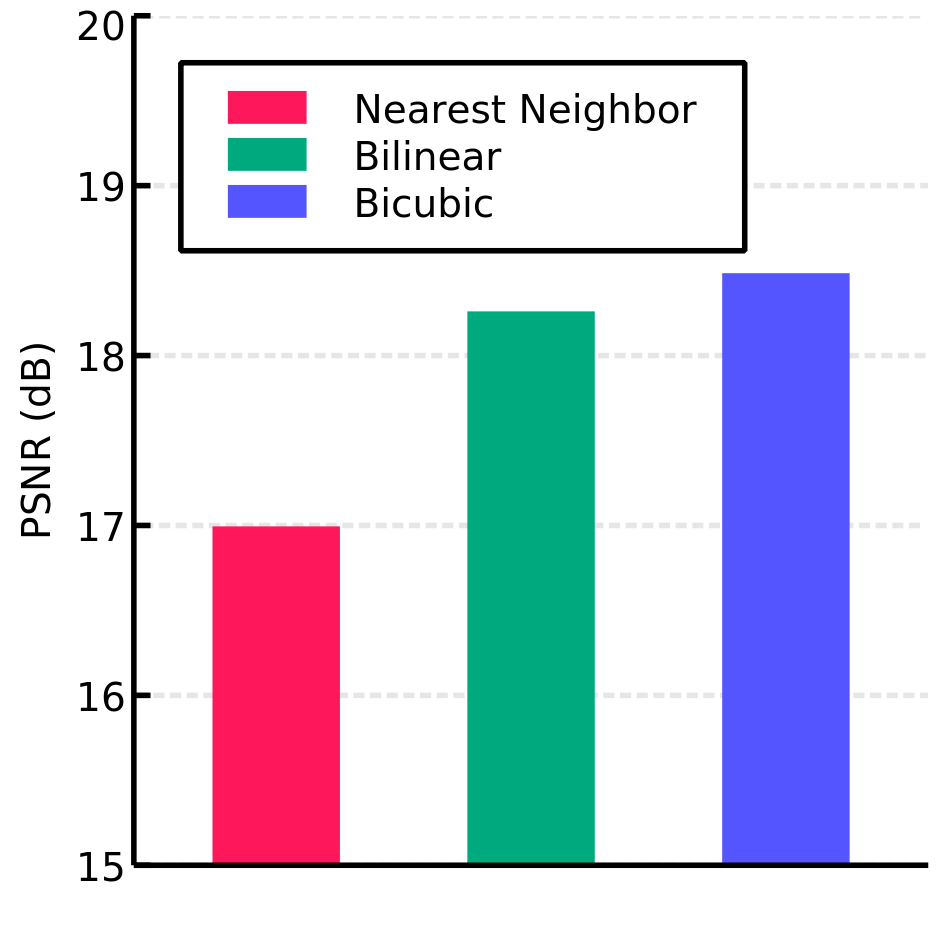
\includegraphics[scale=0.45]{../data/psnr_x4.png}\label{fig:psnrx4}
}
\caption{(a) 영상을 8배 축소후 확대 했을 때, (b) 4배 축소 후 확대 했을 때 각 interpolation 방식에 따른 PSNR.}

\end{figure}

PSNR 를 비교할 경우 위에서 언급한 대로 nearest neighbor 방식이 제일 오차가 크다는 것을 알 수 있다. 또한 bilinear 방식과 bicubic 방식은 큰 차이가 보이지 않으나 수치적으로는 bicubic 방식이 PSNR 이 더 낮게 나온다. 비교를 위해서 8배 축소 후 8배 확대가 아닌 4배 축소 후 4배 확대를 진행해보았는데, Fig.~\ref{fig:psnrx4} 에서 그 결과를 볼 수 있다. 이 경우에는 bicubic 이 bilinear 방식보다 PSNR 이 높게 나왔다. Bicubic 과 bilinear 는 상황에 따라서 우열이 바뀌는 경우가 있는 것으로 추정할 수 있다. 반면에 nearest neighbor 방식은 두 경우 모두에 PSNR 이 가장 낮게 나왔다. 4배 축소 확대를 한 경우에는 영상의 원정보 손실이 상대적으로 작기 때문에 8배로 했을 때보다 전체적인 PSNR 이 높게 나왔다.

\subsection{구현2}
구현2 에서는 제공받은 영상 \code{Right\_arrow.tif} 를 15도 회전시킨 후, 각각 $x$축과 $y$축의 양의 방향으로 10픽셀, 15픽셀 만큼 이동시켰다. 이동시킨 후의 모습은 Fig.~\ref{fig:result2} 와 같다..

\begin{figure}[H]
\centering
\subfigure[Nearest Neighbor]{
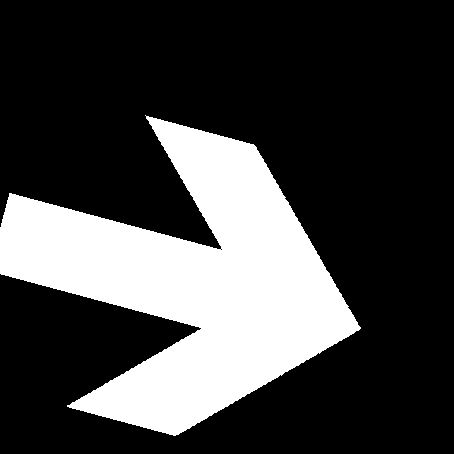
\includegraphics[scale=0.25]{../data/nearest_impl2.png}
}
\subfigure[Bilinear]{

\includegraphics[scale=0.25]{../data/bilinear_impl2.png}
}
\subfigure[Bicubic]{

\includegraphics[scale=0.25]{../data/bicubic_impl2.png}
}
\caption{(a) Nearest neighbor, (b) bilinear, (c) bicubic interpolation 을 사용했을 때의 구현2 결과물.}
\label{fig:result2}
\end{figure}

여기서도 각 interpolation 방법에 따른 차이를 확인할 수가 있는데, 영상들의 경계선을 확대할 경우 명확하게 나타난다. 이러한 차이는 Fig.~\ref{fig:zoom} 에 있다.

\begin{figure}[H]
\centering
\subfigure[Nearest Neighbor]{
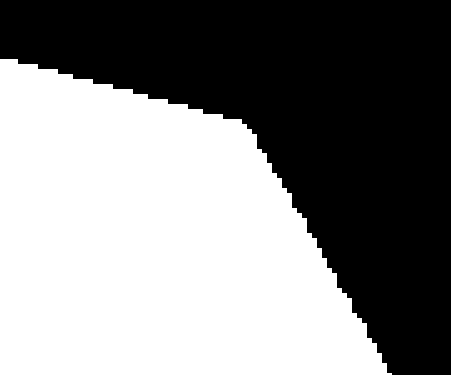
\includegraphics[scale=0.4]{../data/nearest_zoom.png}
}
\subfigure[Bilinear]{
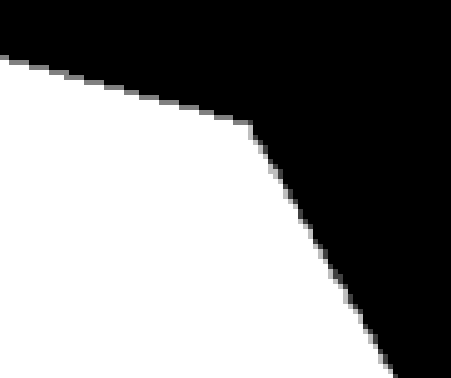
\includegraphics[scale=0.4]{../data/bilinear_zoom.png}
}
\subfigure[Bicubic]{
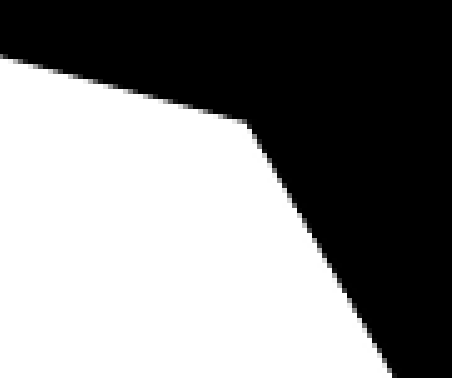
\includegraphics[scale=0.4]{../data/bicubic_zoom.png}
}
\caption{(a) Nearest neighbor, (b) bilinear, (c) bicubic interpolation 을 사용했을 때를 확대한 모습.}
\label{fig:zoom}
\end{figure}

Nearest neighbor 를 사용했을 때 가장자리면이 굉장히 거칠게 형성된다. bilinear 방식을 사용할 때는 이보다는 조금 더 결과물이 부드럽게 보인다. 마지막으로 bicubic 방식을 사용하였을 때 가장 자연스러운 가장자리가 형성된 걸 볼 수 있다. 화살표의 경우에는 정성적으로 판단했을 때 bicubic 방식이 제일 적합하다고 추정할 수 있다.

\section{Conclusion}
이번 과제에서는 affine transformation 을 직접 구현하였고, discrete domain 영상들을 변환하면서 생기는 정보의 손실을 보완하기 위해 interpolation 을 사용하였다. 구현한 interpolation 방식은 nearest neighbor, bilinear, bicubic 이며, 이들의 성능을 간단하게 비교하였다. 영상을 축소하고 다시 확대했을 때 각 interpolation 방식의 성능을 차영상과 PSNR 을 통해서 비교하였다. 또한 회전 및 translation 변환을 했을 때도 각 방식들의 성능 차이를 알아보았다.


\end{document}
